\documentclass[a4paper,10pt]{ltjsarticle}
\usepackage[margin=19mm]{geometry}
\usepackage{amsmath,booktabs,graphicx}
\usepackage[hidelinks]{hyperref}
\title{研究進捗：合成波面の回転補償と単一ポリゴンでの検証}
\author{}
\date{2026年11月28日}
\begin{document}
\maketitle
\section{目的と理論}
各ポリゴンの初期傾斜角を変換式に与えず、保存済みの1枚の複素ホログラムを回転補償できるかを調べる。今回は単一の三角形を対象とした。
従来法は局所キャリアに由来する周波数シフトを含む。先行研究の手法では、共通座標上の物理的な空間周波数ベクトルを回転させる。出力格子 $(u,v)$ から入力の参照位置を求める符号規約で、写像とヤコビアンは
\[
 w=\sqrt{\lambda^{-2}-u^2-v^2},\quad
 \alpha=u\cos\delta+w\sin\delta,\quad \beta=v,\quad
 |J|=\left|\cos\delta-\frac{u}{w}\sin\delta\right|.
\]
回転中心を $(0,0,z_o)$、並進をゼロとした式(14)は
\[
 G_{\rm mc}(u,v;0)=H(u,v;-z_o)\,|J|\,
 H(\alpha,\beta;z_o)G(\alpha,\beta;0),\qquad
 H(u,v;z)=e^{2\pi\mathrm i z w}.
\]
入力をFFTし、参照周波数で補間と回転中心までの伝搬を行い、ヤコビアンを掛けて逆伝搬し、逆FFTで複素ホログラムを得る。入力スペクトルに共通の線形演算なので、合成済みの場にも一括適用できる。固定照明下で物体を回して再生成した波面との一致には別途検証が必要である。出典：\href{https://doi.org/10.1364/OE.27.037383}{Symeonidou et al., Optics Express 27, 37383--37399 (2019), 式(14)}。

\section{条件と画質評価}
各条件で、初期角のOriginal複素配列1枚（$512\times512$）を両方式に共通入力とした。変換式には相対角 $\delta=\theta_{\rm target}-\theta_{\rm input}$ を用いた。画素ピッチは $4.5\,\mu\mathrm{m}$、波長530\,nm、回転中心距離 $z_o=2$\,mm、ゼロパディング後 $1024\times1024$、Cubic補間、帯域外はゼロ。符号は比較実験で採用した規約である。

\begin{center}\small
\begin{tabular}{lrrrrr}\toprule
条件（度）&\multicolumn{2}{c}{従来法}&\multicolumn{2}{c}{式(14)}&式(14) 帯域外\\
&PSNR [dB]&SSIM&PSNR [dB]&SSIM&格子点率\\\midrule
$0\to0$&217.68&1.000&219.03&1.000&0.0\%\\
$45\to45$&217.20&1.000&216.22&1.000&0.0\%\\
$0\to1$&31.48&0.879&21.33&0.810&14.8\%\\
$0\to-1$&33.24&0.907&21.70&0.856&14.8\%\\
$30\to29$&31.38&0.924&22.39&0.859&14.8\%\\
$45\to44$&29.53&0.913&22.72&0.870&14.8\%\\
$45\to42$&23.13&0.868&16.39&0.775&44.4\%\\
$45\to40$&20.29&0.832&8.25&0.552&74.1\%\\\bottomrule
\end{tabular}
\end{center}
PSNR・SSIMはホログラム面の振幅を目標角Originalの範囲で正規化して算出した。式(14)のゼロ回転の複素相対誤差は最大 $4.3\times10^{-11}$。非ゼロ角の6条件では従来法の振幅指標が高かった。帯域外参照率は出力格子点の割合であり、失われたエネルギーの割合とは区別する。

\clearpage
\section{1枚の入力から得た変換結果}
45度のOriginalを1枚入力し、相対角$-1$度を指定した。同じ44度のOriginalと比較すると、式(14)のホログラム振幅PSNRは22.72\,dB、SSIMは0.870、複素相対誤差 $\|g-g_{\rm ref}\|_F/\|g_{\rm ref}\|_F$ は1.405、出力と入力のFrobeniusノルム比は0.9996であった。
\begin{center}
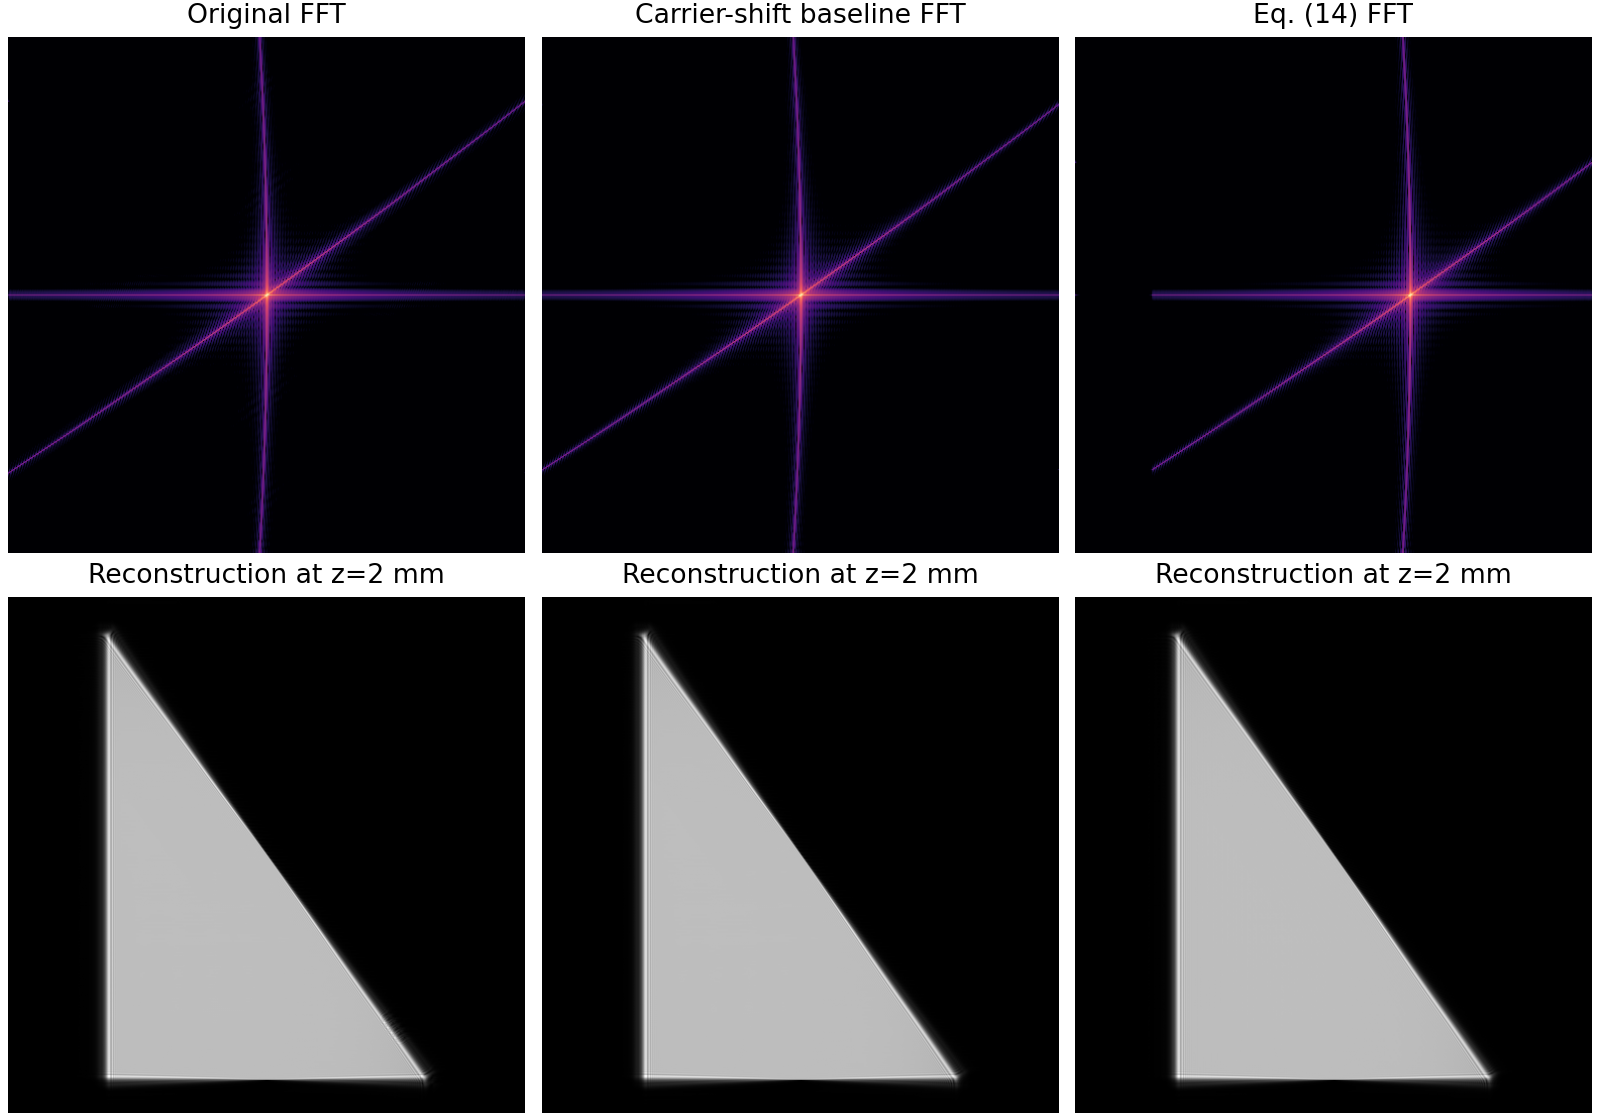
\includegraphics[width=\linewidth]{figures/comparison.png}
\end{center}
上段は複素ホログラムのFFT振幅、下段は2\,mm伝搬した再生振幅。左から目標角のOriginal、従来法、式(14)である。式(14)のFFTはスペクトルの分布位置が移動する一方、再生像には三角形の輪郭が残る。

式(14)の写像では $\alpha(0,0)=\sin\delta/\lambda$ となる。今回の \(\pm111.11\,\mathrm{mm}^{-1}\) の帯域では、原点の参照位置は約3.38度で端に達する。45度から40度の条件では出力と入力のノルム比が0.0293まで低下した。複素誤差は位相やキャリアの差にも反応するため、再生輪郭のずれと併せて評価する。

\clearpage
\section{Originalとの輪郭の重ね合わせ}
\begin{center}
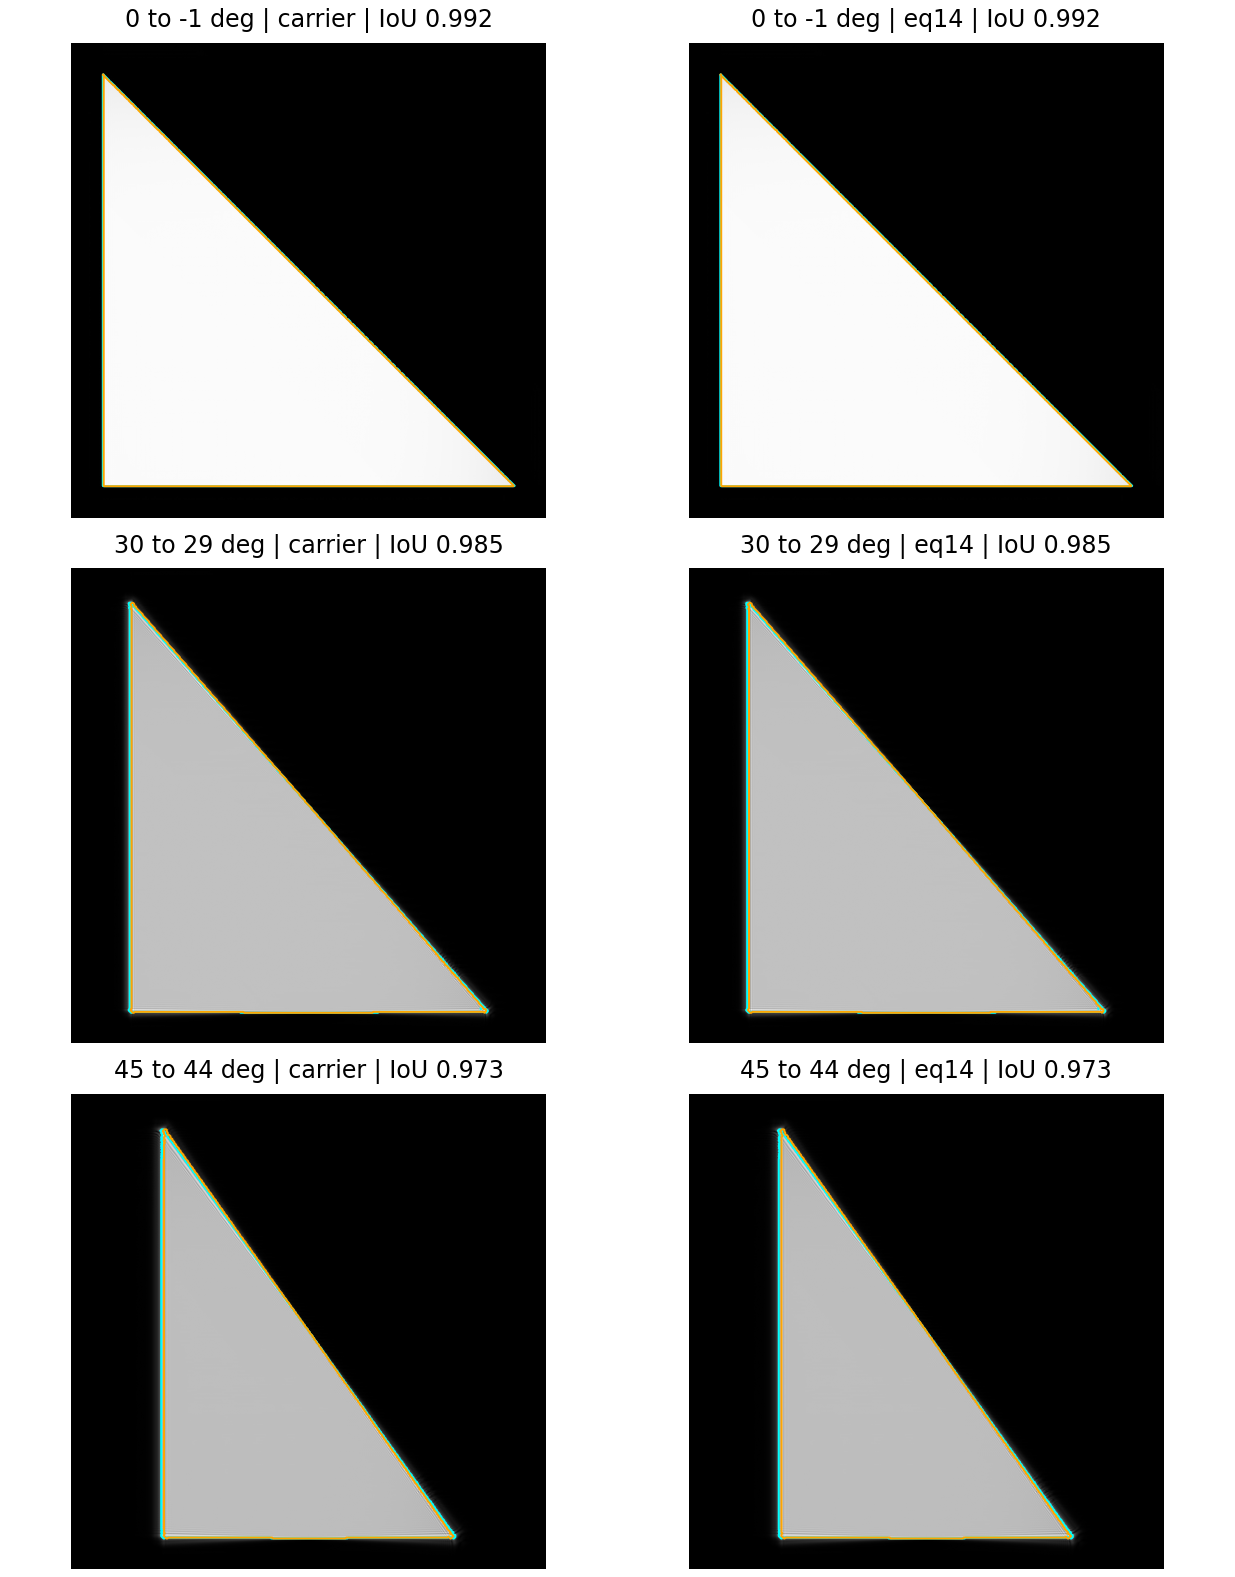
\includegraphics[height=.68\textheight,keepaspectratio]{figures/overlay.png}
\end{center}
背景と水色の輪郭はOriginal、橙色の輪郭は変換結果。各条件のOriginal再生振幅の最大値の50\%を共通閾値とし、位置合わせをせず同一画素座標で比較した。IoUは二値領域の共通部分と和集合の面積比である。

\begin{center}\small
\begin{tabular}{lrrrr}\toprule
条件（度）&\multicolumn{2}{c}{従来法}&\multicolumn{2}{c}{式(14)}\\
&IoU&重心距離 [px]&IoU&重心距離 [px]\\\midrule
$0\to-1$&0.992&0.72&0.992&0.72\\
$30\to29$&0.985&0.70&0.985&0.70\\
$45\to44$&0.973&1.10&0.973&1.09\\\bottomrule
\end{tabular}
\end{center}
同じ$-1$度の3条件では、式(14)でも輪郭の重なりは大きかった。一方、複素波面の一致は確認できていない。次は回転の符号と照明・キャリアの規約を照合し、複素誤差の要因を切り分ける。全条件の数値は \texttt{metrics.csv}、輪郭比較は \texttt{overlay\_metrics.csv} に保存した。
\end{document}
